\documentclass[12pt]{scrartcl}
\usepackage[sexy]{james}
\usepackage[noend]{algpseudocode}
\setlength {\marginparwidth}{2cm}
\usepackage{answers}
\usepackage{array}
\usepackage{tikz}
\newenvironment{allintypewriter}{\ttfamily}{\par}
\usepackage{listings}
\usepackage{xcolor}
\usetikzlibrary{arrows.meta}
\usepackage{color}
\usepackage{mathtools}
\newcommand{\U}{\mathcal{U}}
\newcommand{\E}{\mathbb{E}}
\usetikzlibrary{arrows}
\Newassociation{hint}{hintitem}{all-hints}
\renewcommand{\solutionextension}{out}
\renewenvironment{hintitem}[1]{\item[\bfseries #1.]}{}
\renewcommand{\O}{\mathcal{O}}
\declaretheorem[style=thmbluebox,name={Chinese Remainder Theorem}]{CRT}
\renewcommand{\theCRT}{\Alph{CRT}}
\setlength\parindent{0pt}
\usepackage{sansmath}
\usepackage{pgfplots}

\usetikzlibrary{automata}
\usetikzlibrary{positioning}  %                 ...positioning nodes
\usetikzlibrary{arrows}       %                 ...customizing arrows
\newcommand{\eqdef}{=\vcentcolon}
\newcommand{\tr}{{\rm tr\ }}
\newcommand{\im}{{\rm Im\ }}
\newcommand{\spann}{{\rm span\ }}
\newcommand{\Col}{{\rm Col\ }}
\newcommand{\Row}{{\rm Row\ }}
\newcommand{\dint}{\displaystyle\int}
\newcommand{\dt}{\ {\rm d }t}
\newcommand{\PP}{\mathbb{P}}
\newcommand{\horizontal}{\par\noindent\rule{\textwidth}{0.4pt}}
\usepackage[top=3cm,left=3cm,right=3cm,bottom=3cm]{geometry}
\newcommand{\mref}[3][red]{\hypersetup{linkcolor=#1}\cref{#2}{#3}\hypersetup{linkcolor=blue}}%<<<changed

\tikzset{node distance=4.5cm, % Minimum distance between two nodes. Change if necessary.
         every state/.style={ % Sets the properties for each state
           semithick,
           fill=cyan!40},
         initial text={},     % No label on start arrow
         double distance=4pt, % Adjust appearance of accept states
         every edge/.style={  % Sets the properties for each transition
         draw,
           ->,>=stealth',     % Makes edges directed with bold arrowheads
           auto,
           semithick}}


% Start of document.
\newcommand{\sep}{\hspace*{.5em}}

\pgfplotsset{compat=1.18}
\begin{document}
\title{AMSC460: Homework 4}
\author{James Zhang\thanks{Email: \mailto{jzhang72@terpmail.umd.edu}}}
\date{\today}

\definecolor{dkgreen}{rgb}{0,0.6,0}
\definecolor{gray}{rgb}{0.5,0.5,0.5}
\definecolor{mauve}{rgb}{0.58,0,0.82}

\lstset{frame=tb,
  language=Java,
  aboveskip=3mm,
  belowskip=3mm,
  showstringspaces=false,
  columns=flexible,
  basicstyle={\small\ttfamily},
  numbers=left,
  numberstyle=\tiny\color{gray},
  keywordstyle=\color{blue},
  commentstyle=\color{dkgreen},
  stringstyle=\color{mauve},
  breaklines=true,
  breakatwhitespace=true,
  tabsize=3
}

\maketitle

\begin{center}
  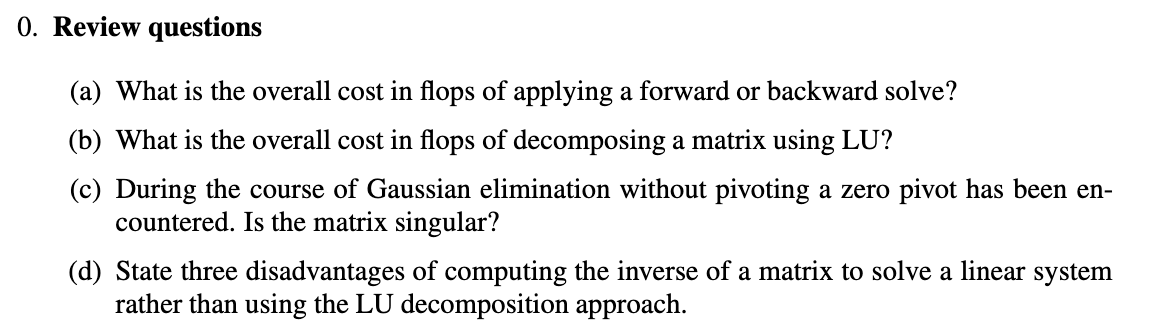
\includegraphics[width=14cm]{0.png}
\end{center}

\begin{proof}[Solution]
  \hfill

  \begin{enumerate}[(a)]
    \item The overall cost in flops for forward or backward solving is $\mathcal{O}(n^2)$. 
    \item The overall cost in flops for decomposing a matrix using LU is $\mathcal{O}(n^3)$. 
    \item No. If we encounter a zero pivot during the course of Gaussian Elimination, this does not always mean that the matrix is singular --- we can interchange the rows. 
    See \textbf{Example 5.7} in the textbook for a counterexample. 
    \item Three advantages to using a LU Decomposition approach over a matrix inverse approach are 
    \begin{enumerate}[1.]
      \item Finding the inverse of a matrix is an inefficient, wasteful use of storage. 
      \item Finding the inverse of a matrix --- while also an $\mathcal{O}(n^3)$ algorithm --- is more computationally expensive than finding the LU Decomposition, though by less than an order of magnitude. 
      \item Finding the inverse of a matrix is more prone to larger roundoff errors than the LU Decomposition. Finding the inverse also has no advantages to outweigh the disadvantages. 
    \end{enumerate}
  \end{enumerate}
\end{proof}

\newpage 

\begin{center}
  
\includegraphics[width=14cm]{1.png}
\end{center}

\begin{proof}[Solution]
  The above system yields the following augmented matrix, which we will perform Gaussian Elimination on in order 
  to obtain an upper triangular matrix. 
  \[\begin{bmatrix}
    1 & -1 & 3 & \vline & 2\\
    1 & 1 & 0 & \vline & 4\\
    3 & -2 & 1 & \vline & 1
  \end{bmatrix} \xrightarrow{R_1 - R_2, \ \& \ R_1 - \frac{1}{3}R_3}
  \begin{bmatrix}
    1 & -1 & 3 & \vline & 2\\
    0 & -2 & 3 & \vline & -2\\
    0 & -\frac{1}{3} & \frac{8}{3} & \vline & \frac{5}{3}
  \end{bmatrix}\]
  \[\xrightarrow{R_2 - 6R_3}
    \begin{bmatrix}
      1 & -1 & 3 & \vline & 2\\
      0 & -2 & 3 & \vline & -2\\
      0 & 0 & -13 & \vline & -12
    \end{bmatrix}\]
    and this is our resulting upper triangular matrix. Now applying backwards substitution, we get immediately that 
    \[-13x_3 = -12 \implies x_3 = \frac{12}{13}\] Now plugging this value in for the next equation, we solve 
    \[-2x_2 + 3(\frac{12}{13}) = -2 \implies -2x_2 = -\frac{62}{13} \implies x_2 = \frac{31}{13}\]
    Finally, solving for the last unknown $x_1$, 
    \[x_1 - \frac{31}{13} + 3(\frac{12}{13}) = 2 \implies x_1 = 2 + \frac{31}{13} - \frac{36}{13} \implies x_1 = \frac{21}{13}\]
    Therefore, using Gaussian Elimination and Backwards Substitution, we arrive at our solution \[\vec{\textbf{x}} = \begin{bmatrix}
      x_1\\x_2\\x_3
    \end{bmatrix} = 
    \begin{bmatrix}
      \frac{21}{13}\\ \frac{31}{13} \\ \frac{12}{13}
    \end{bmatrix}\]
\end{proof}

\newpage

\begin{center}
  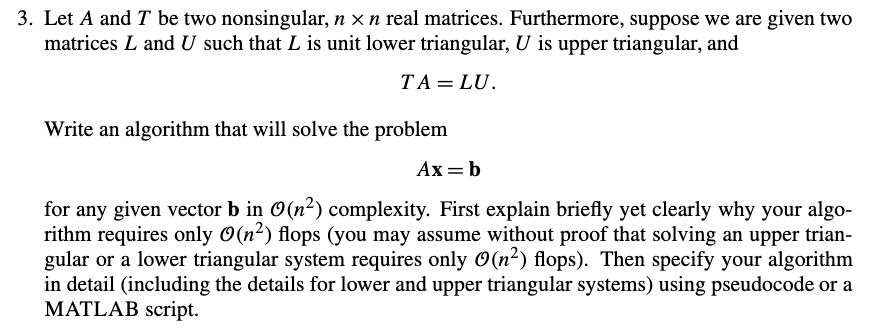
\includegraphics[width=14cm]{3.png}
\end{center}

\begin{proof}
  Note that in the following steps, we are not computing the inverse of $T$ in MATLAB, but rather we are doing this to develop a new algorithm and rewrite our givens. 
  Let $T^{-1}$ be the matrix inverse of $T$ and observe that 
  \[TA = LU \implies T^{-1}TA = T^{-1}LU \implies A = T^{-1}LU\]
  Substitute this into the equation $Ax=b$, and we get that 
  \[T^{-1}LUx = b\]
  Now left multiply both sides by $T$, and we are left with 
  \[TT^{-1}LUx = Tb \implies LUx = Tb\]
  where $Tb$ is a new vector. Let $y = Ux$, which yields 
  \[Ly = Tb\]
  and we can then solve for $y$ using forward substitution. Once we have $y$, we can solve 
  \[Ux = y\]
  for $x$ using backward substitution, and we will have obtained our answer. 
  
  \hfill
  
  \textbf{Time Complexity}: Note that the matrix multiplication $Tb$, forward substitution, and 
  backward substitution are all $\mathcal{O}(n^2)$, and so our entire algorithm's time complexity is $\mathcal{O}(n^2)$. 
  \begin{lstlisting}[language=Matlab]
% Given A, T, L, U, and b.
Tb = T * b;
% Forward Substitutution. 
for k = 1:n
  y(k) = (Tb(k) - L(k, 1:k-1) * y(1:k-1)) / L(k, k);
end
% Backwards Substitution. 
x(n) = y(n) / U(n,n);
for k = n-1:-1:1
  x(k) = (y(k) - U(k,k+1:n) * x(k+1:n)) / U(k,k);
end
  \end{lstlisting}
\end{proof}

\end{document}

